\documentclass[svgnames]{beamer}
\mode<presentation>
\usefonttheme{serif}
\usecolortheme{dove}
\useinnertheme{rounded}
%\useoutertheme{smoothbars}
\setbeamercolor{item projected}{fg=black}
\setbeamertemplate{navigation symbols}{}

\usepackage{times}
\usepackage[french]{babel}
\usepackage{amsthm,amssymb,amsmath,graphicx}
\usepackage{color}
\usepackage{gastex}
\usepackage{framed}
\usepackage{graphicx}
\usepackage{multicol}
\usepackage{ulem}
\usepackage{ifthen}
\usepackage{tikz}
\usepackage{appendixnumberbeamer}
\usepackage{eurosym}

%%%%%%%%%%%%%%%%%%%%%%%%%%%%%%%%%%%%%%%%%%%%%%%%%%%%%%%%%%%%%%%%%%%%%%%%%%%%%%%%%%%%%%%%
%%%%%%%%%%%%%%%%%%%% A non-original creation by Nathanaël Fijalkow and Victor Marsault %

\setbeamertemplate{frametitle}{
  \vskip-2pt
  \begin{beamercolorbox}[rightskip=2cm,leftskip=1em,dp=1ex,wd=12.8cm]{frametitle}
    \vskip2pt
    \usebeamercolor{frametitle}
    \begin{tikzpicture}
      \useasboundingbox (0,0) rectangle (0,0); 
      \ifthenelse{\insertframenumber<\inserttotalframenumber}
      { 
        \pgfmathsetmacro{\aimangle}{90-(\insertframenumber*360/\inserttotalframenumber)}
        \fill [fill=frametitle.fg,thin, color=gray!50,draw=black] (11.8,.2) -- (11.8,.6) arc (90:\aimangle:0.4) -- cycle;

      }{ 
        \fill[fill=frametitle.fg,thin, color=gray!50,draw=black] (11.8,0.2) circle (.4);
      }
      \fill[fill=frametitle.fg,thin, color=white,draw=black] (11.8,0.2) circle (.3);
      \node at (11.8, .2) [black,circle]{\normalsize\insertframenumber};
    \end{tikzpicture}
    \insertframetitle
    \vskip2pt
  \end{beamercolorbox}
}
%%%%%%%%%%%%%%%%%%%%%%%%%%%%%%%%%%%%%%%%%%%%%%%%%%%%%%%%%%%%%%%%%%%%%%%%%%%%%%%%%%%%%%%

\setbeamertemplate{blocks}[rounded]
\setbeamercolor{block title}{bg=normal text.bg!90!black}
\setbeamercolor{block body}{bg=normal text.bg!95!black}

\newcommand{\A}{\mathcal{A}}
\newcommand{\Q}{\mathbb{Q}}
\newcommand{\N}{\mathbb{N}}
\newcommand{\tr}[1]{\langle #1 \rangle}
\newcommand{\prob}[1]{\mathbb{P}_{#1}}
\newcommand{\set}[1]{\{ #1 \}}
\newcommand{\val}[1]{\text{val}(#1)}
  
\title{
Bourse CNRS Momentum \\
\vskip1em
\textbf{Deep Synthesis} \\
\textit{Apprentissage pour la Synth{\`e}se de Programmes}
\textbf{Dur{\'e}e} : Jan. 2019 - D{\'e}c. 2021 (3 ans) \\
\textbf{Budget} : 180k \euro
}
\subtitle{Nathana{\"e}l Fijalkow}
\institute{

\includegraphics[height=3cm]{Fig/CNRS}
\hspace*{1cm}

\includegraphics[height=3cm]{Fig/LaBRI}
\hspace*{1cm}

\includegraphics[height=3cm]{Fig/Turing}
}
\date{}

\begin{document}

\addtocounter{framenumber}{-1}

\begin{frame}
  \titlepage
\end{frame}

\begin{frame}{Qu'est-ce que la synth{\`e}se (en m{\'e}thodes formelles) ?}

La \textcolor{magenta}{synth{\`e}se} est une proc{\'e}dure :
\begin{itemize}
	\item \textbf{Entr{\'e}e} : \textcolor{red}{sp{\'e}cification} (compl{\`e}te ou partielle)
	\item \textbf{Sortie} : un \textcolor{blue}{syst{\`e}me} r{\'e}alisant la sp{\'e}cification
\end{itemize}

\vskip1em
Trois types de syst{\`e}mes :

\begin{center}

\includegraphics[height=2.5cm]{Fig/code}
\hspace*{.2cm}
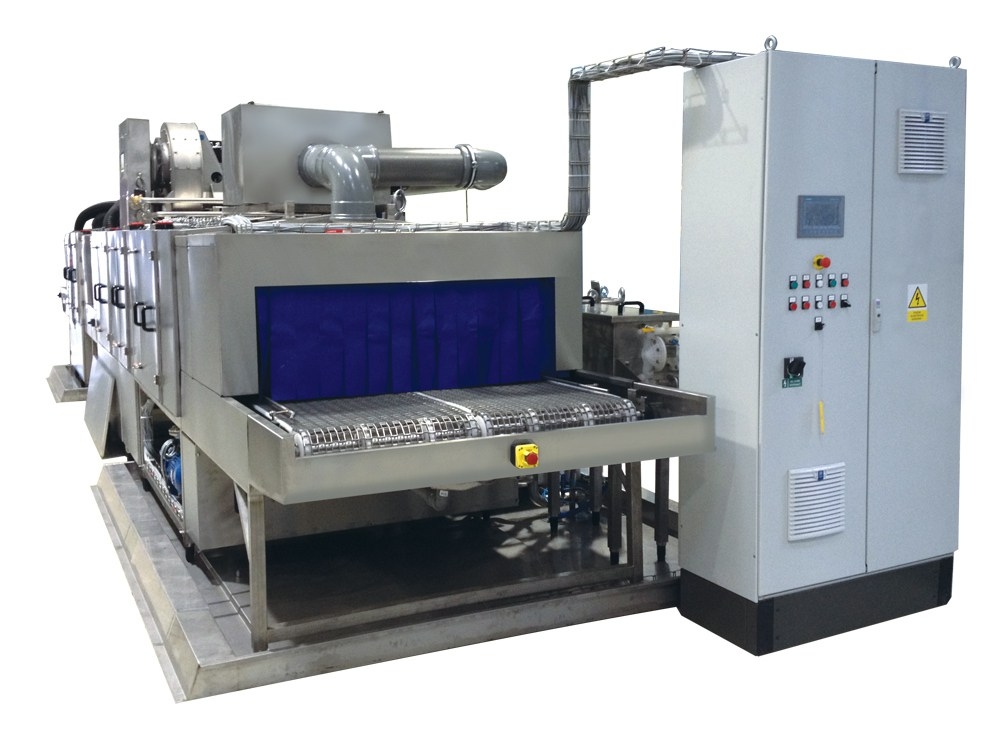
\includegraphics[height=2.5cm]{Fig/machine}
\hspace*{.2cm}
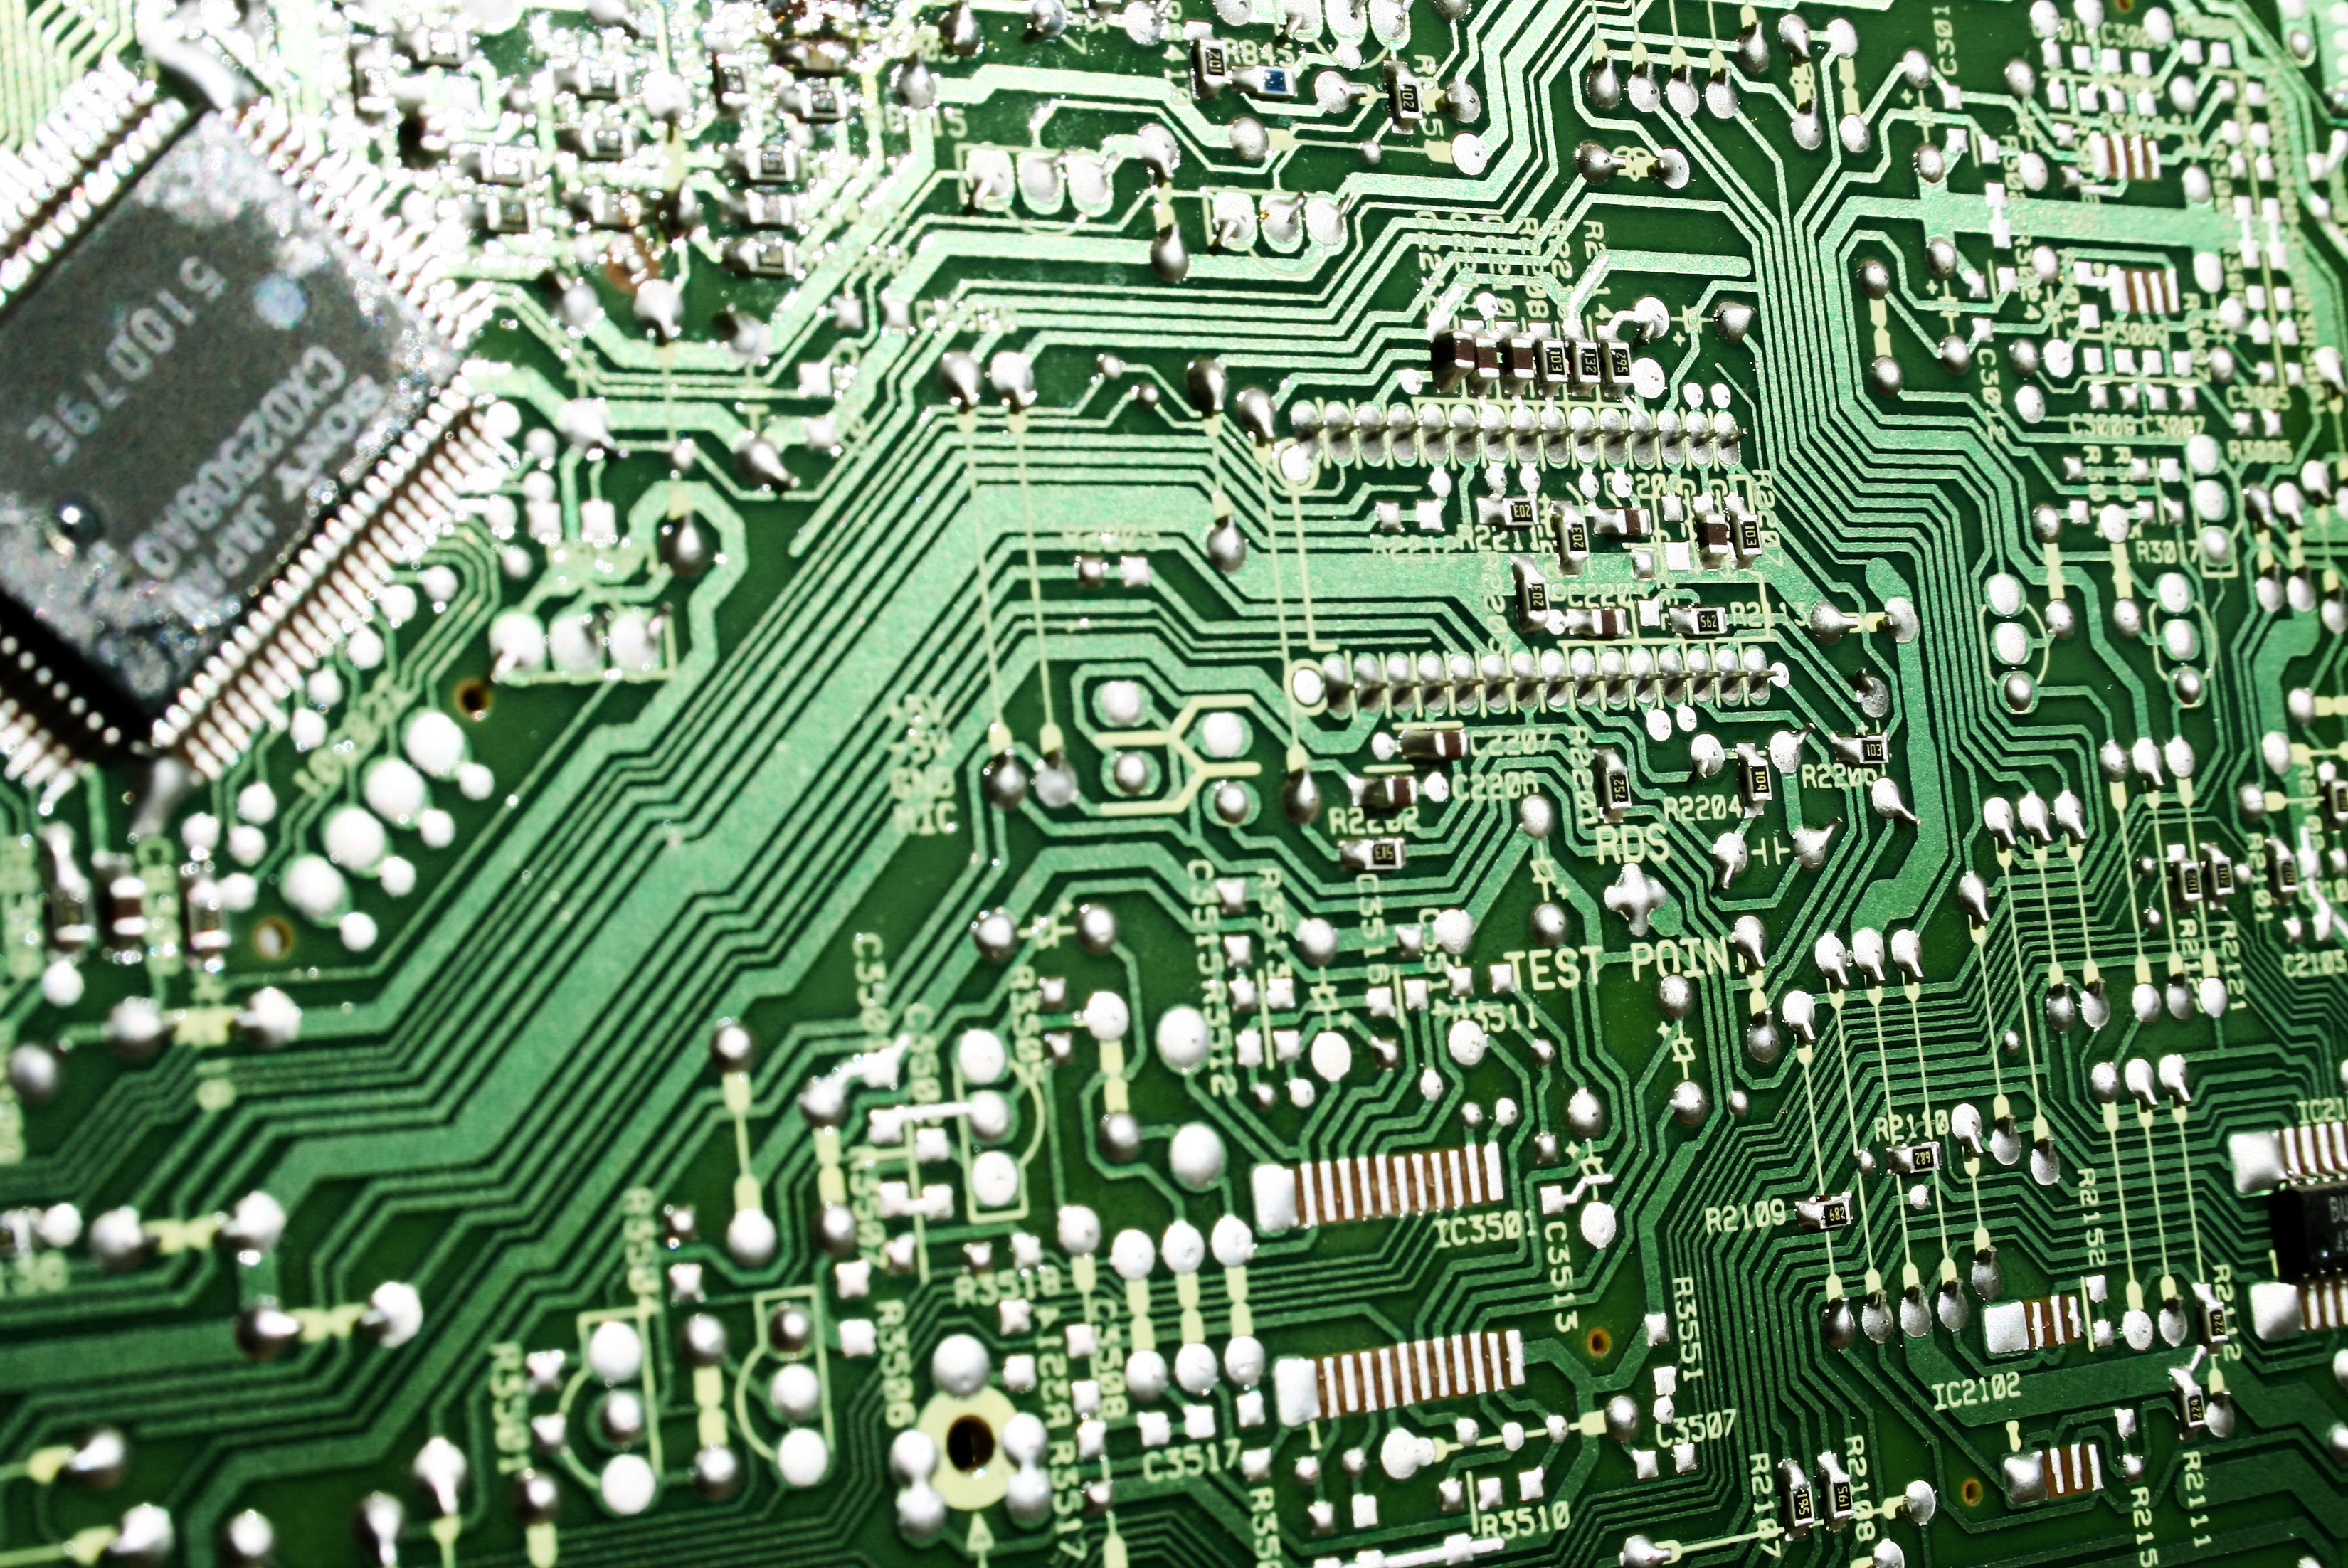
\includegraphics[height=2.5cm]{Fig/electronique}

programme \hspace{6em} contr{\^o}leur \hspace{6em} composante
\end{center}
\end{frame}

\begin{frame}{D{\'e}roulement du projet DeepSynth}
\textbf{Deux axes}
\begin{itemize}
	\item \textcolor{red}{Jeux de parit{\'e}} : synth{\`e}se du $\mu$-calcul modal

	\textbf{Objectif} : \textit{Construire des algorithmes efficaces pour les jeux de parit{\'e} en s'appuyant sur des
m{\'e}thodes d'apprentissage}

	\item \textcolor{blue}{Processus de d{\'e}cisions markoviens} : syst{\`e}mes probabilistes,	base du reinforcement learning
	
	\textbf{Objectif} : \textit{{\'E}tudier la notion de strat{\'e}gie implantable}	
\end{itemize}

\vskip1em

\textbf{Calendrier}
\begin{itemize}
	\item \textbf{2019} : d{\'e}veloppements th{\'e}oriques et m{\'e}thodologiques,
	identification des potentielles applications

	\item \textbf{2020-2021} : embauche d'un post-doctorant pour travailler sur le premier axe,
	implantation des algorithmes et tests {\`a} diff{\'e}rentes {\'e}chelles
\end{itemize}
\end{frame}

\end{document}
